\section{Questions}

\begin{frame}
    \frametitle{Questions}

    \begin{itemize}
        \item What are algorithms?
        \item Why is the study of algorithms worthwhile?
        \item What is the role of algorithms relative to other technologies used in computers?
    \end{itemize}

\end{frame}

\section{Algorithms}

\begin{frame}
    \frametitle{What are algorithms?}

    \begin{itemize}
        \item Informally, an \emph{algorithm} is any well-defined \underline{computational procedure} (计算过程) that takes some value, or set of values, as \emph{input} and produces some value, or set of values, as \emph{output} in \underline{a finite amount of time}.
        \item  An algorithm is thus a sequence of computational steps that transform the input into the output.
    \end{itemize}

\end{frame}

\begin{frame}
    \frametitle{Example: compute the square root of a number}

    \begin{enumerate}
        \item Start with a guess, $g$.
        \item If $g \times g$ is close enough to $x$, stop and say that $g$ is the answer.
        \item Otherwise, create a new guess by averaging $g$ and $\frac{x}{g}$, i.e., $\frac{(g + \frac{x}{g})}{2}$.
        \item Using this new guess, which we again call $g$, repeat the process until $g \times g$ is close enough to $x$.
    \end{enumerate}

\end{frame}

\begin{frame}
    \frametitle{An algorithm is like a recipe from a cookbook}

    材料:肉丝 1 把,白菜 1 片,较小洋葱 1 个,水发木耳 2 大朵,红尖椒半个,姜丝 1 小撮,葱段适量。

    调料:淀粉 1 汤勺,盐、料酒、味精、生抽适量,香油 1 小勺。
    \begin{enumerate}
        \item 肉丝、淀粉、一点点料酒混合抓匀。白菜洗净、擦干,裁去叶留帮,切成5厘米长的段,顺菜筋改刀成0.5厘米宽的丝;木耳切丝;洋葱去外皮,洗净切丝;红尖椒纵切丝。
        \item 炒锅里放油烧至七八成热,保持中火,放入姜丝和肉丝,用铲子拨散,肉丝发白时加入生抽翻炒。
        \item 看生抽色裹住肉丝时,放入白菜和木耳,翻炒1分钟,放入洋葱丝、红尖椒丝翻炒,待洋葱丝稍软关火,放盐、味精、香油、葱段拌匀盛盘。
    \end{enumerate}

\end{frame}

\begin{frame}
    \frametitle{A formal defined sorting problem}

    \emph{Input}: A sequence of $n$ number $\left\langle a_1, a_2, \cdots, a_n \right\rangle$

    \emph{Output}: a permutation (reordering) $\left\langle a_1', a_2', \cdots, a_n'\right\rangle$ of the input sequence such that $a_1' \leqslant a_2'\leqslant \cdots \leqslant a_n'$.

    \pause
    \vspace{\baselineskip}

    Given the input sequence $\left\langle 31, 41, 59, 26, 41, 58 \right\rangle$, a \emph{correct} sorting algorithm returns as output the sequence $\left\langle 26, 31, 41, 41, 58, 59 \right\rangle$

\end{frame}

\begin{frame}
    \frametitle{Correct algorithm}

    \begin{itemize}
        \item An algorithm for a computational problem is \emph{correct} if, for every problem instance provided as input, it \emph{halts}, finishes its computing in finite time, and outputs the \underline{correct solution} to the problem instance.
    \end{itemize}

\end{frame}

\begin{frame}
    \frametitle{What kinds of problems are solved by algorithms?}

    \begin{figure}
        \centering
        
\includegraphics[width = \linewidth]{./ch/images/ch1/01_human_genome_project.jpg}
    \end{figure}

\end{frame}

\begin{frame}
    \frametitle{What kinds of problems are solved by algorithms?}

    \begin{figure}
        \centering
        \includegraphics[width = \linewidth]{./ch/images/ch1/02_networks.pdf}
    \end{figure}

\end{frame}

\begin{frame}
    \frametitle{What kinds of problems are solved by algorithms?}

    \begin{figure}
        \centering
        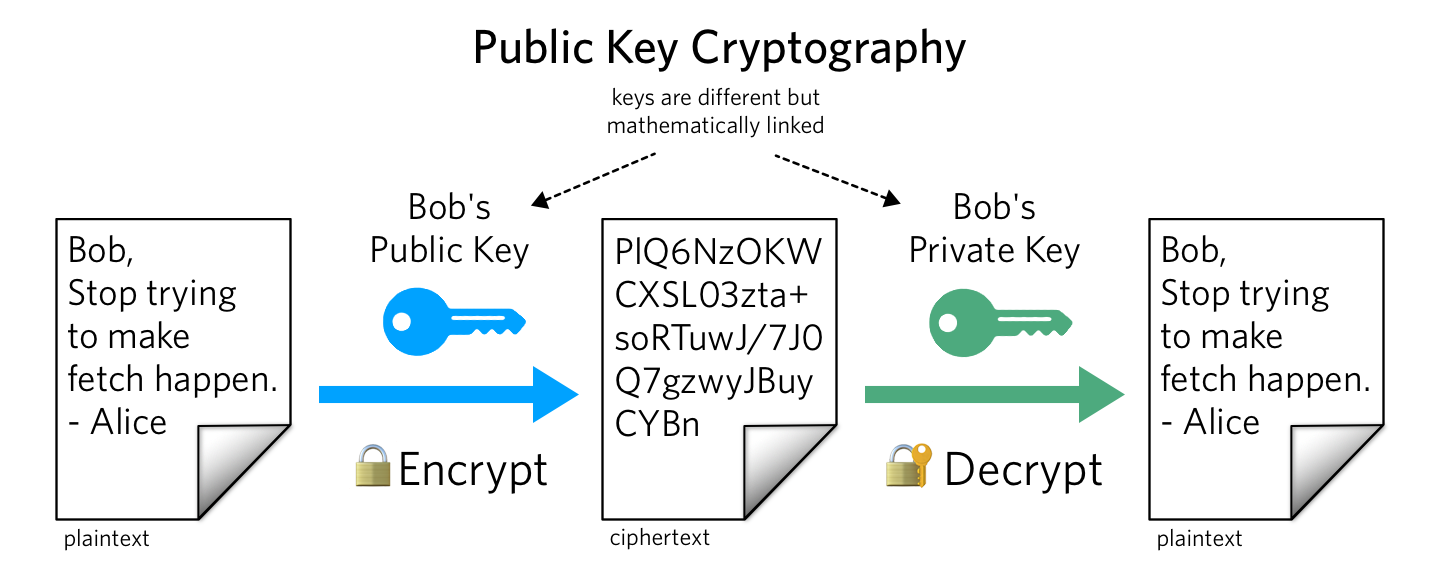
\includegraphics[width = \linewidth]{./ch/images/ch1/03_public_key_cryptography.png}
    \end{figure}

\end{frame}

\begin{frame}
    \frametitle{What kinds of problems are solved by algorithms?}

    \begin{figure}
        \centering
        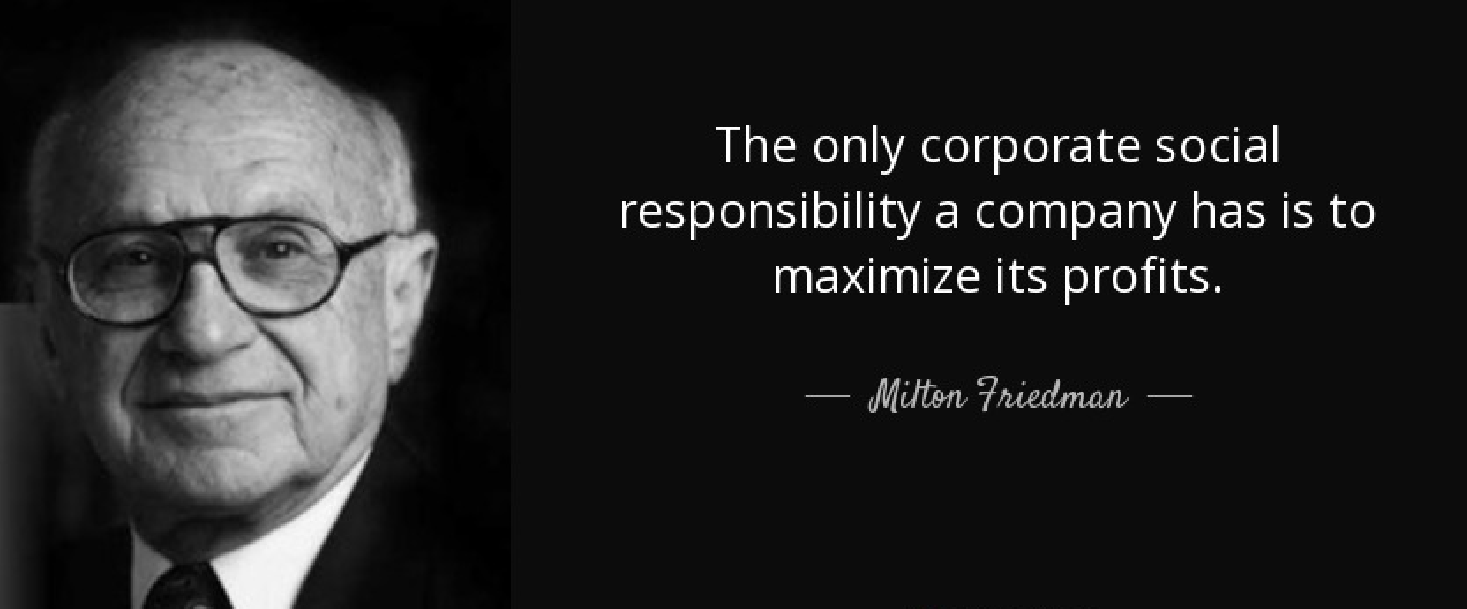
\includegraphics[width = \linewidth]{./ch/images/ch1/04_max_profit.png}
    \end{figure}

\end{frame}